\documentclass{article}
\setlength{\oddsidemargin}{0.25 in}
\setlength{\evensidemargin}{-0.25 in}
\setlength{\topmargin}{-0.6 in}
\setlength{\textwidth}{6.5 in}
\setlength{\textheight}{8.5 in}
\setlength{\headsep}{0.75 in}
\setlength{\parindent}{0 in}
\setlength{\parskip}{0.1 in}

% ===== PACKAGES =====
\usepackage{amsmath,amssymb}
\usepackage{color}
\usepackage{subfigure}
\usepackage{mdframed}
\usepackage{changepage}
\newmdenv[
  topline=false,
  bottomline=false,
  skipabove=\topsep,
  skipbelow=\topsep
]{siderules}
\renewcommand{\abstractname}{}

% ===== VARIABLES =====
\def \R{\mathbb{R}}
\def \Pr{\mathbb{P}}
\def \D{{\rm D}}
\def \N{{\rm N}}
\def \xx{{\boldsymbol{\rm x}}}
\def \y{{\rm y}}




% ===== HEADER BOX =====
\newcommand{\lecture}[2]{
\pagestyle{myheadings}
\thispagestyle{plain}
\newpage
\noindent
\begin{center}
\rule{\textwidth}{1.6pt}\vspace*{-\baselineskip}\vspace*{2pt} % Thick horizontal line
\rule{\textwidth}{0.4pt}\\[1\baselineskip] % Thin horizontal line
\vbox{\vspace{2mm}
\hbox to 6.28in { {\bf CS 760: Machine Learning} \hfill Spring 2024 }
\vspace{4mm}
\hbox to 6.28in { {\Large \hfill #1  \hfill} }
\vspace{4mm}
\hbox to 6.28in { {\scshape Authors:}  #2 \hfill }}
\vspace{-2mm}
\rule{\textwidth}{0.4pt}\vspace*{-\baselineskip}\vspace{3.2pt} % Thin horizontal line
\rule{\textwidth}{1.6pt}\\[\baselineskip] % Thick horizontal line
\end{center}
\vspace*{4mm}
}

% ===== Jed's Defined Stuff ======
\DeclareMathOperator*{\argmin}{arg\!\min}
\DeclareMathOperator*{\argmax}{arg\!\max}
\usepackage{siunitx}
\usepackage{enumitem} % used to make alphabetical lists instead of numbered ones
\usepackage{mathtools}
\usepackage{graphicx}
\usepackage{caption}
\usepackage{hyperref}


% =============== DOCUMENT ===============
\begin{document}
\lecture{Convolutional Neural Networks}{Jed Pulley \& Keshav Sharan Pachipala}

\begin{center}
{\Large {\sf \underline{\textbf{DO NOT POLLUTE!}} AVOID PRINTING, OR PRINT 2-SIDED MULTIPAGE.}}
\end{center}

% \begin{abstract}
% Write your abstract here
% \end{abstract}

\section{Introduction}
    In recent years, Convolutional Neural Networks (CNNs) have emerged as a cornerstone technology in the field of deep learning, particularly in the domain of computer vision. CNNs are adept at extracting intricate patterns and features from spatially structured data. Some fields that benefit from CNNs include image classification, object detection, and medical image analysis.
    
    In this paper, we won't go into the exact specifics of what a convolution is since it's slightly different in the discrete and continuous cases, as well as slightly different in a CNN context, but if you're really curious about it, 3Blue1Brown has some excellent videos visually explaining the mathematical concepts behind a convolution in his videos linked below [1] and [2].

\section{Understanding the Architecture}
    \subsection{NNs vs CNNs}
        Neural Networks and CNNs are similar in many ways, but also have drastically different architectures. From a high level, the classic neural network example has an input layer, hidden layers, and an output layer, shown below:
        
        \begin{center}
            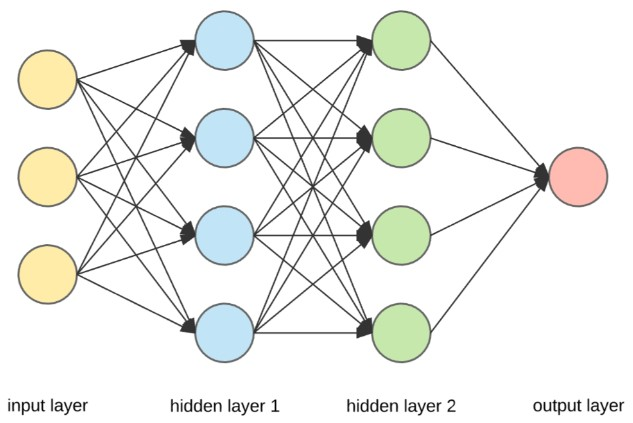
\includegraphics[scale=0.5]{images/NN.jpg}    
        \end{center}
        
        However, the architecture of a convolution neural network looks much different. There isn't one right way to structure it, but typically a CNN will have the input, a few convolution and pooling layers, a flattening step, and then finally a fully connected layer that leads to an output, as shown below. Notably, how you structure your CNN is an area of active research today.
        
        \begin{center}
            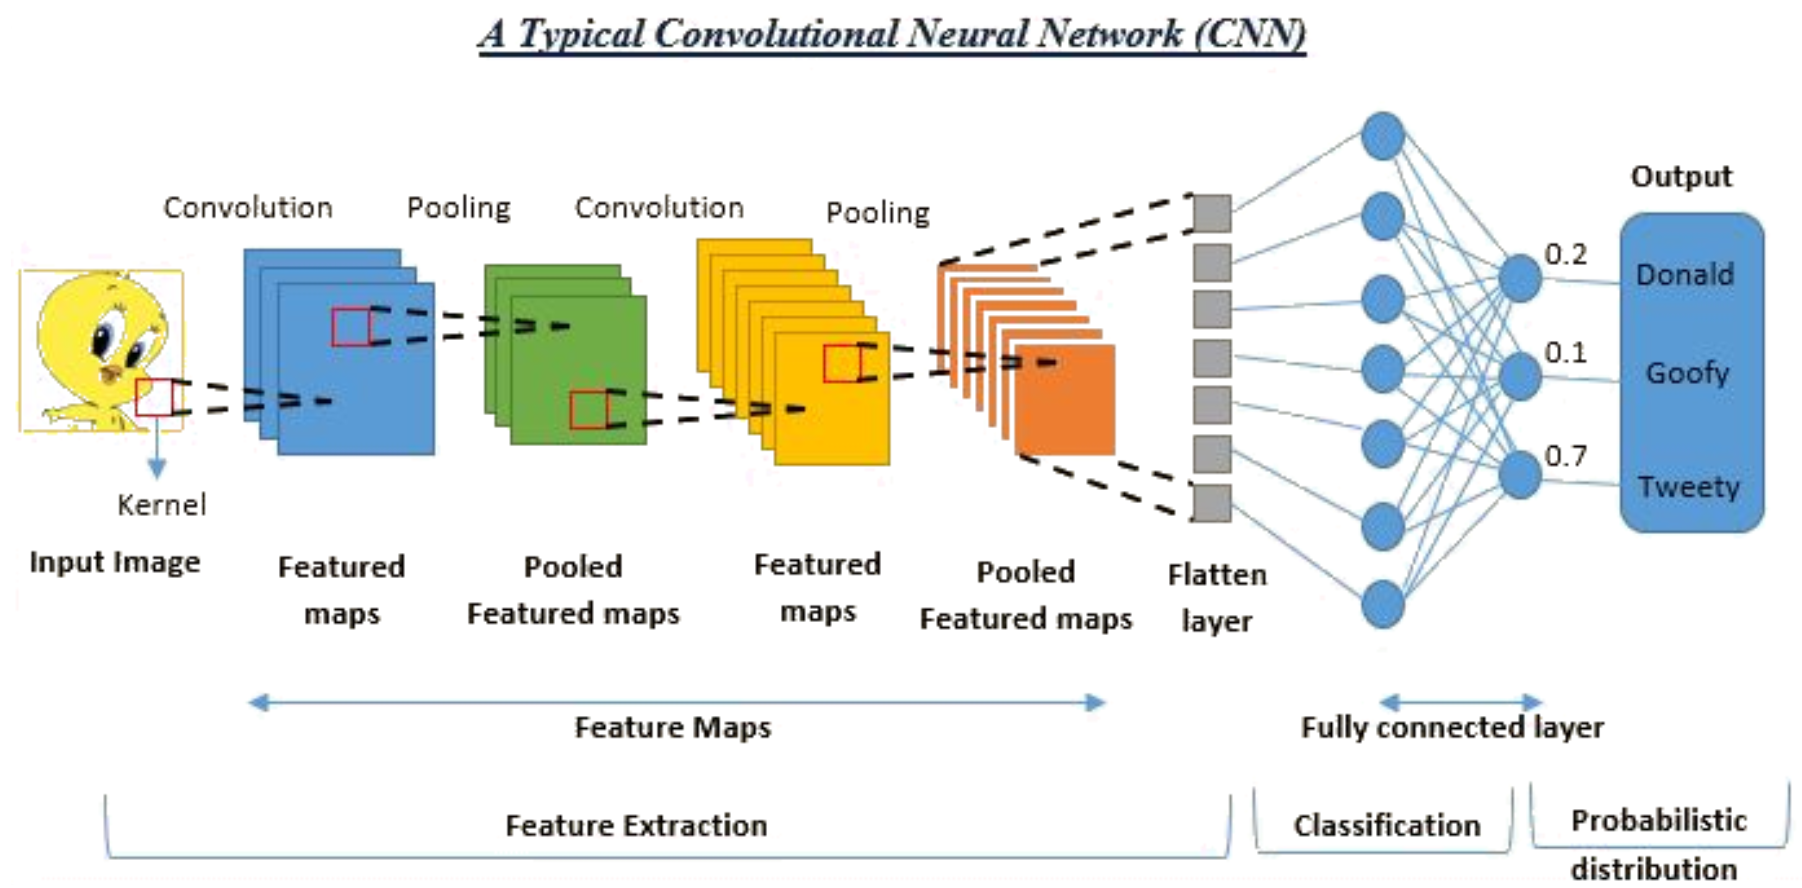
\includegraphics[scale=0.3]{images/CNN.jpg}
        \end{center}
        
        Another important distinction between the two is that for a CNN, the weights that we are trying to learn are the kernels themselves, along with a bias term.

    \subsection{Kernels}
        Fundamental to the idea of convolutions are kernels. In the context of CNNs, the words kernel and filter are interchangeable, but for this paper we'll stick with kernel. In the 2D image processing case, a kernel takes the form of a square grid of odd dimensions. So for example 3x3, 5x5, or 9x9. These days, you'll almost exclusively see kernels of dimensions 3x3 or even 1x1. Kernels are odd so that they have a center. The reason for 3x3 goes back to 2012 when the ImageNet competition was in full swing. Briefly put, ImageNet was a challenge to see who could most efficiently and accurately classify a dataset of more than 14 million hand-annotated images into roughly 20,000 categories. In 2012, a model called AlexNet swept the competition outperforming all others by significant margins. AlexNet pioneered CNNs for the image processing task. One of the reason's for it's success was it's heavy use of 3x3 kernels. However, it wasn't until the next year when an optimized version of AlexNet, called ZFNet, took it a step further and used 3x3 kernels in almost every layer. There are many different ways to determine your kernel size, but starting out with 3x3 is a safe bet.
        
    \subsection{Convolution Layer}
        The convolution layer is the defining aspect of a CNN. To actually perform the convolution step means sliding the kernel across the image pixel by pixel, multiplying each element with it's overlapping counterpart, summing them up, and then dividing them by the kernel size (3x3 having a size of 9). The output is a single pixel in the output image/matrix. You scroll through the entire image performing the same operation until complete. This step is shown in the image below:
        
        \begin{center}
            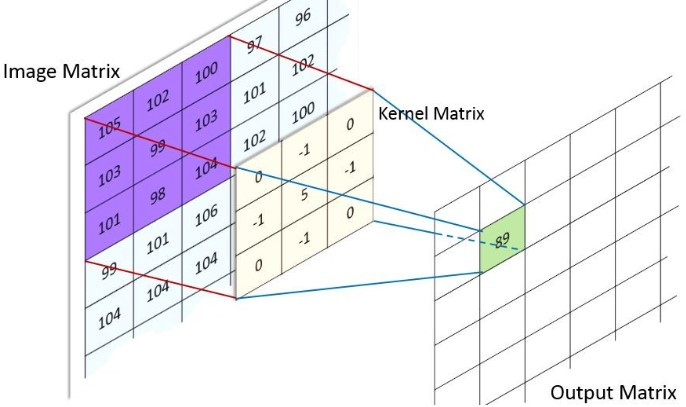
\includegraphics[scale=0.6]{images/kernel.jpg}
        \end{center}
        
        Since the operative pixel is the center of the kernel, convolution runs into the issue of overlapping the image. So to avoid this, with a 3x3 kernel for example, a single pixel of padding is added to the image so that the kernel will fit in the first row/column.

        The general expression for a convolution is as follows:
        \[ g(x, y) = \omega \ast f(x, y) = \sum_{i=-a}^{a} \sum_{j=-b}^{b} w(i, j) * f(x - i, y - j) \]
        where $g(x, y)$ is the filtered image, $f(x, y)$ is the original image, and $\omega$ is the kernel.

        One of the biggest advantages of a convolution is that when applied to structured data, it can take advantage of the spatial relationship between said data. Whereas normally that relationship would be lost when flattened out and pumped through a regular neural net.

    \subsection{Pooling Layer}
        The next step of the CNN is to perform pooling on the input image. There are many methods used for this, but the most common are max pooling and average pooling. For pooling, you again take a kernel (this one doesn't need to have odd dimensions) and scan it across the image. However this time, instead of going pixel by pixel, you stride over the image. And for each step, in the max pooling case, you take the maximum value in the overlapping kernel region:
        
        \begin{center}
            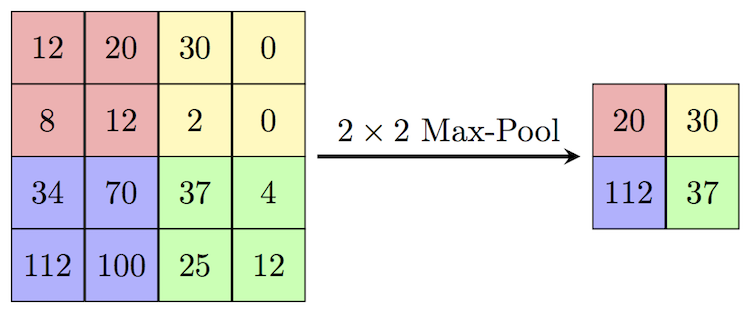
\includegraphics{images/maxpool.png}
        \end{center}
        
        In the case of average pooling, the process is exactly the same excpet instead of taking the maximum, you average the values out and use that. Often times, you'll see a kernel size of 2x2 and a "stride" of 2 for pooling. This means that you'll examine a 2x2 area, choose the maximum (or average) of that area, and then return it. After that, you stride the kernel over two steps and repeat over the entire image. This has two main functions: down sampling and shift-invariance
        
        \begin{enumerate}
            \item Down Sampling: This step reduces the overall size of your data while also preserving the main features from the previous layers. So moving forward, you are left with a smaller, more informationally dense input that gets propagated into further layers. This leads to more computational efficiency.
            \item Shift-Invariance: This effect is slightly less stated, but still important. If, for example, the kernel's job was to detect whiskers on a cat, down-sampling makes the convolution step slightly more invariant to shifts in the image. Since pooling carries forward important features and reduces the area, you get the same feature but are less concerned with where in the image that feature was found. This effect is marginal, but still leads to more robust classification.
        \end{enumerate}

    \subsection{Flattening \& Fully Connected Layer}
        The flattening step appears after the convolutional and pooling layers. It acts as a bridge between the convolutional/pooling layers, which extract spatial features, and the fully connected layers, which perform classification or regression tasks. After flattening, a fully connected layer is hooked up to the output layer with it's own weights and biases.
        
    \subsection{Output Layer}
        The output layer is the same as what you would find in a regular neural network. For a classification task, the outputs would be the confidence of that specific class. However, this layer is generalizable to the specific needs of whatever flavor of CNN you are implementing.

    \subsection{Activation Functions}
        Like any neural network, CNNs use activation functions to introduce non-linearity into the system. Common activation functions include Tanh, ReLU, and the Sigmoid functions, as shown below:

        \textbf{Sigmoid}
        \[ \sigma(z) = \frac{1} {1 + e^{-z}} \]

        \textbf{ReLU}
        \[ Relu(z) = max(0, z) \]

        \textbf{Tanh}
        \[ tanh(x) = \frac{e^x - e^{-x}}{e^x + e^{-x}} = \frac{1 - e^{-2x}}{1 + e^{-2x}} \]

    \subsection{Batch Normalization}
        To quote from Younesi et al. [4]:

        \begin{quote}
            Batch Normalization is a technique that helps stabilize and accelerate the training of CNNs. It normalizes the activations of each layer by centering and scaling the values using the mean and variance of each mini-batch during training. This process reduces internal covariate shifts, making the optimization process smoother and enabling the use of higher learning rates. By normalizing activations, Batch Normalization allows for more aggressive learning rates, which leads to faster convergence and improved model generalization. Additionally, it acts as a regularizer, reducing the need for other regularization techniques like dropout. Overall, Batch Normalization has become a standard component in CNN architectures, contributing to faster training, improved model performance, and increased ease of hyperparameter tuning. Its widespread adoption has significantly contributed to the success of modern CNNs in various CV and NLP applications.
        \end{quote}

    \subsection{Backpropagation}
        Unlike traditional neural networks, both the forward pass and the backprop pass of a convolutional layer are convolutions [5].

        I don't want to go into further detail as my explanation would pale in comparison to Pavithra Solai's explanation in the article linked at [5] below. If you're interested in an excellent visual and intuitive understanding of CNN backprop, I highly recommend it.
        
\section{Advanced CNN Architectures}
    \subsection{VGGNet}
        \begin{center}
            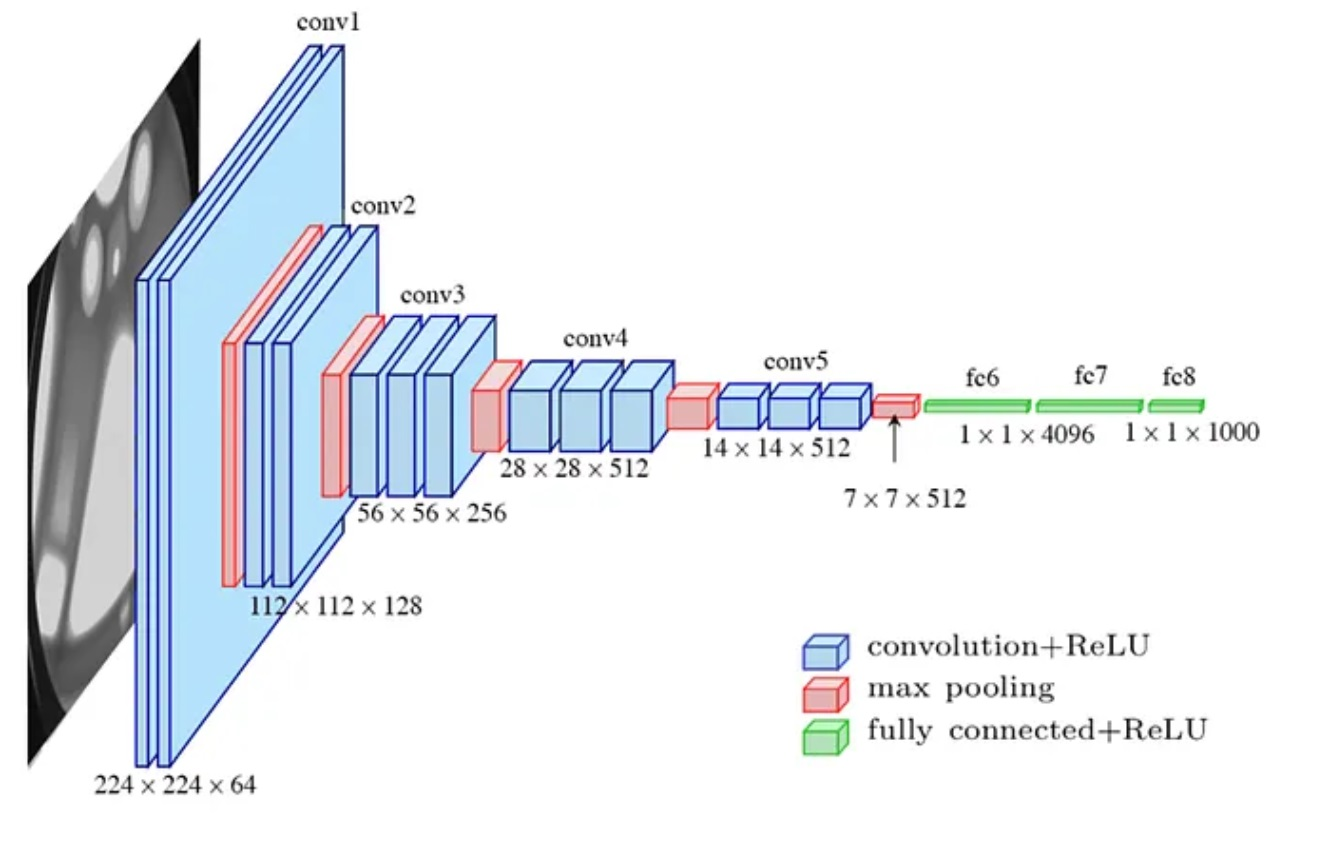
\includegraphics[scale=0.4]{images/VGG.jpg}
        \end{center}

    \subsection{GoogleNet (Inception Net)}
        \begin{center}
            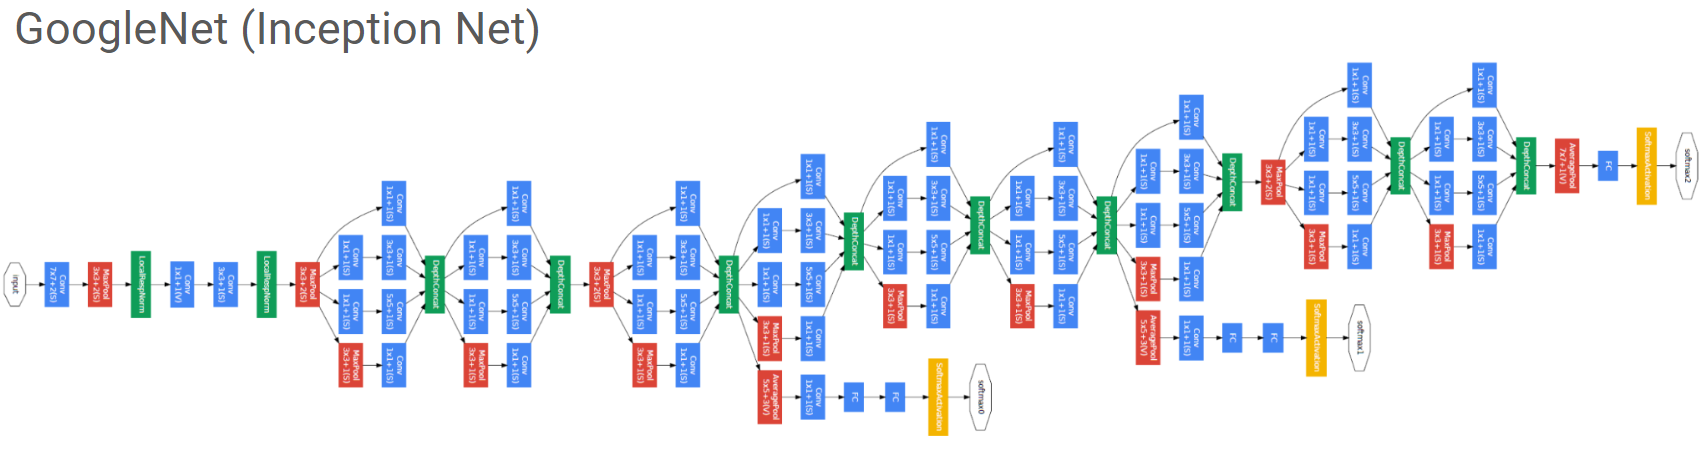
\includegraphics[scale=0.35]{images/GoogleNet.png}
        \end{center}

    \subsection{ResNet}
        \begin{center}
            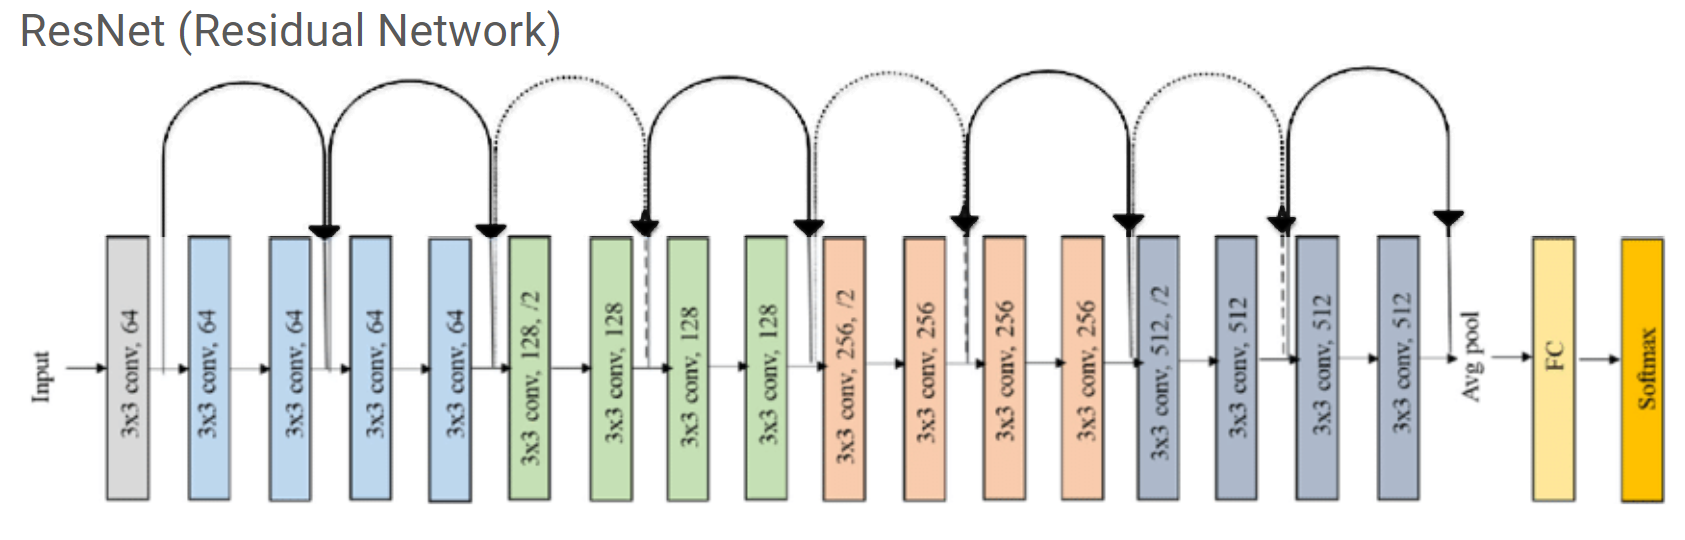
\includegraphics[scale=0.35]{images/ResNet.png}
        \end{center}

\section{Future Directions and Trends}
    \subsection{Accuracy}
        \begin{center}
            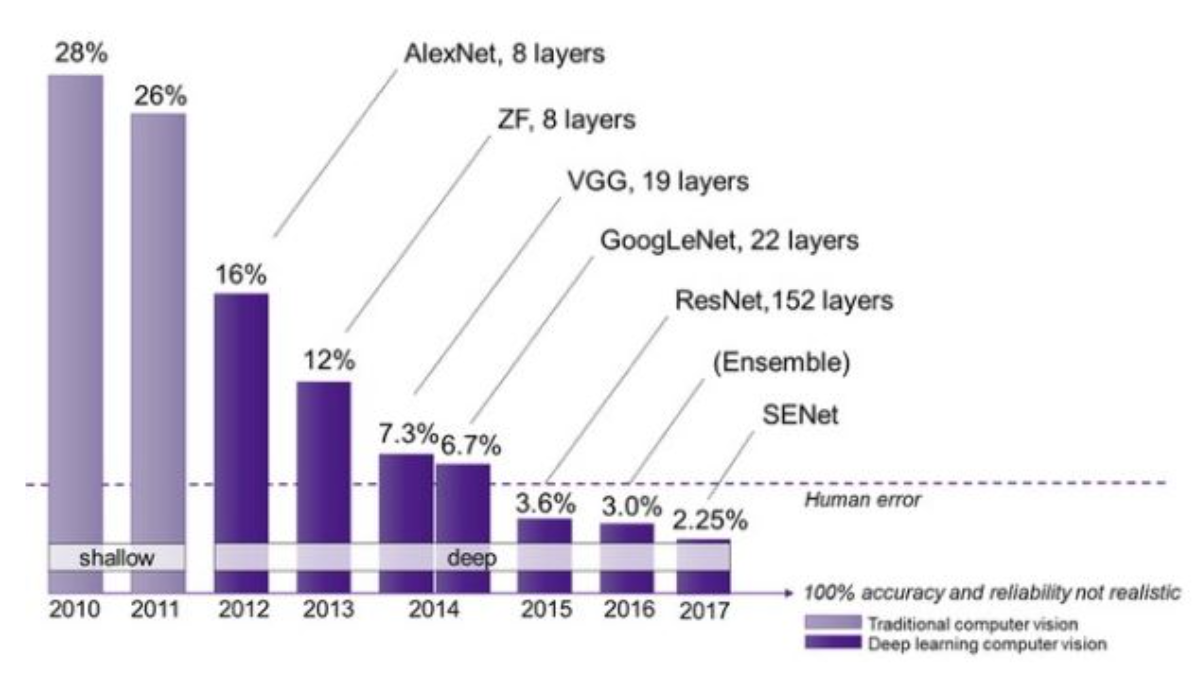
\includegraphics[scale=0.35]{images/accuracy.png}
        \end{center}

    \subsection{Potential Improvements}
        \begin{itemize}
            \item \textbf{Efficiency and Optimization}: Streamline CNNs to require fewer computational resources to enable deployment on low-power devices.
            \item \textbf{Robustness and Generalization}: Increase CNNs’ resilience to adversarial attacks and their ability to perform well on unseen data.
            \item \textbf{Transfer Learning and Few-Shot Learning}: Adapt CNNs to new tasks with minimal data through methods like transfer and few-shot learning.
            \item \textbf{Interpretability and Explainability}: Make CNN decisions transparent and understandable to ensure trustworthiness and compliance in critical applications.
        \end{itemize}
    

\section{Resources}
    \textbf{[1]} 3Blue1Brown - But What is a Convolution? \\
    \url{https://www.youtube.com/watch?v=KuXjwB4LzSA&t=1s}
    
    \textbf{[2]} 3Blue1Brown - Convolutions | Why X+Y in probability is a beautiful mess \\
    \url{https://www.youtube.com/watch?v=IaSGqQa5O-M}
    
    \textbf{[3]} far1din - Convolutional Neural Networks from Scratch | In Depth \\
    \url{https://www.youtube.com/watch?v=jDe5BAsT2-Y}
    
    \textbf{[4]} Younesi, A., Ansari, M., Fazli, M. A., Ejlali, A., Shafique, M., \& Henkel, J. (2024). A Comprehensive Survey of Convolutions in Deep Learning: Applications, Challenges, and Future Trends. arXiv preprint arXiv:2402.15490 \\
    \url{https://arxiv.org/abs/2402.15490}

    \textbf{[5]} Pavithra Solai - Convolutions and Backpropagations \\
    \url{https://pavisj.medium.com/convolutions-and-backpropagations-46026a8f5d2c}


\end{document}